
\section{Results}\label{sec:target_of_the_project} 
Follow the project results plots described in previous section. 
\subsection{Feature Selection}\label{subsec:status}
Power spectral density over time plots obtained from DataProcessing class.
\begin{figure}
\begin{tabular}{cc}

    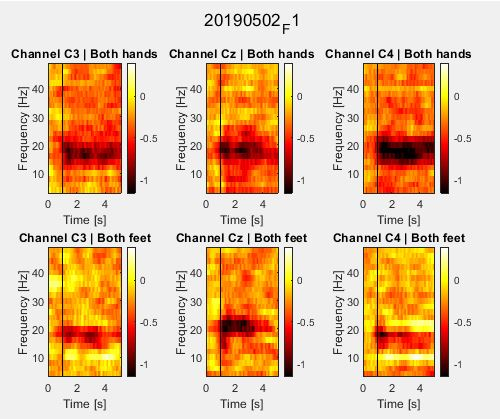
\includegraphics[width=0.5\textwidth]{Figure/20190502_ERDERS.JPG} &   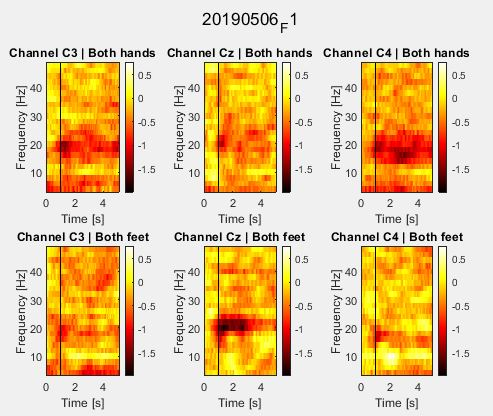
\includegraphics[width=0.5\textwidth]{Figure/20190506_ERDERS.JPG} \\
    (a) 20190502 & (b) 20190506 \\
    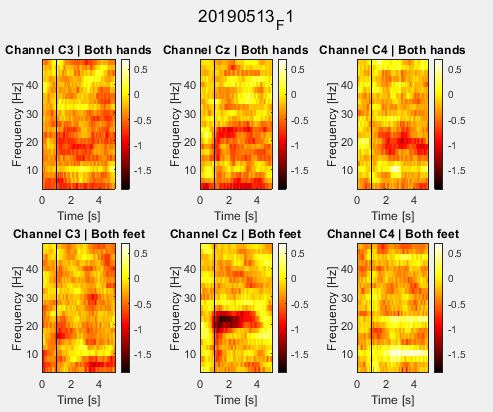
\includegraphics[width=0.5\textwidth]{Figure/20190513_ERDERS.JPG} &   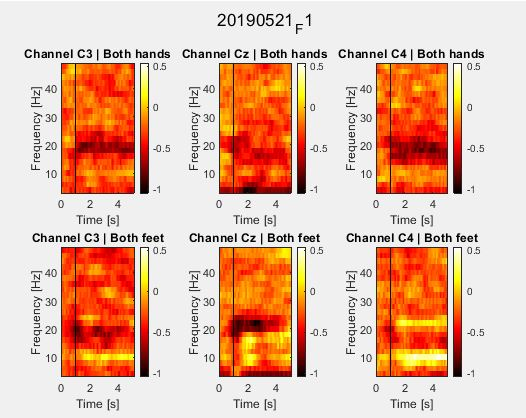
\includegraphics[width=0.5\textwidth]{Figure/20190521_ERDERS.JPG} \\
    (c) 20190513 & (d) 20190521 \\
    \multicolumn{2}{c}{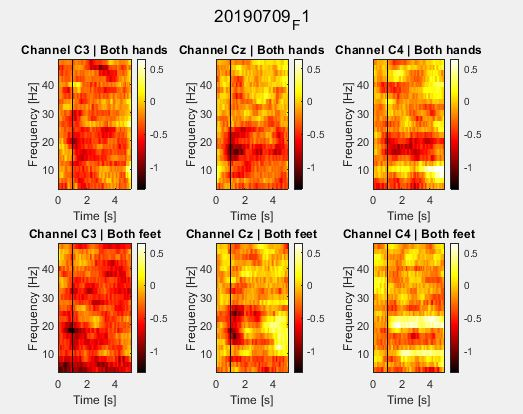
\includegraphics[width=0.5\textwidth]{Figure/20190709_ERDERS.JPG} }\\
    \multicolumn{2}{c}{(e) 20190709}\\


\end{tabular}
\caption{PSD Plots}
\end{figure}

\subsection{Fisher Score results}\label{subsec:status}
From the fisher score result is possible to highlight good discriminant between desired imagery motor in frequency 22Hz and from FC2 and C4 signals. Considering single case we can consider other frequencies like 20Hz and 18Hz and Channels Like FCZ. But this discriminant are present only in some runs, differently from C4,FC2 on 22Hz that are almost present in each offline calibration sessions. (Figure 4)

\subsection{Classifiers}\label{subsec:status}
Follows the classifier results after training. Obviously we have a better discriminant on classifiers that result strong in Channels FC2,C4 on 22Hz during fisher score analysis. This is the proof that this frequency and channels is not the better choice for all sessions. (Figure 5)

\subsection{Single Classifier}\label{subsec:status}
Just for check I tried to create a single classifier using all offline sessions data, the resulting output is very bad. The pilot change on each run and the classifier of first session is completely useless on last sessions. In fact the plot show a total overlap of the features without the possibility to find a good global discriminant (Figure 3)

\subsection{Test Sessions}\label{subsec:status}
Plot of posterior probabilities over time, with 0.7 threshold, that help to understand evidence accumulation.


\begin{figure}[h]
    \centering
    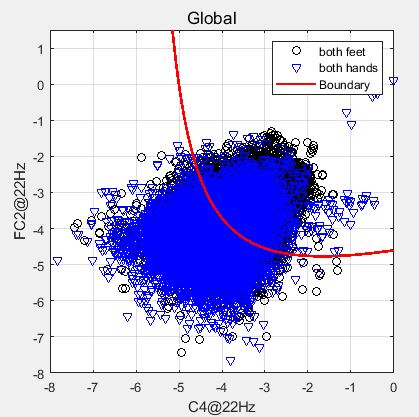
\includegraphics[width=0.5\textwidth]{Figure/GLOBAL_C.JPG}
    \caption{Single classifier.}
    \label{fig:Pipeline}
\end{figure}

\begin{figure}
\begin{tabular}{cc}
    \multicolumn{2}{c}{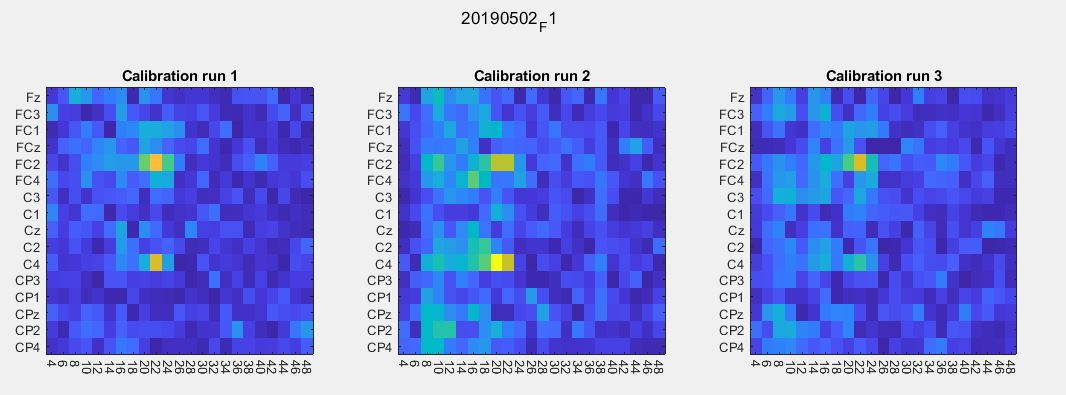
\includegraphics[width=1\textwidth]{Figure/20190502_FS.JPG} }\\
    \multicolumn{2}{c}{(a) 20190502}\\
    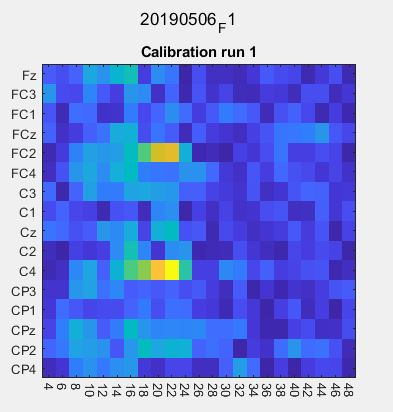
\includegraphics[width=0.5\textwidth]{Figure/20190506_FS.JPG} &   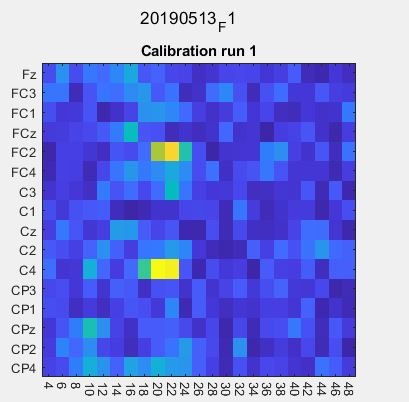
\includegraphics[width=0.5\textwidth]{Figure/20190513_FS.JPG} \\
    (b) 20190506 & (c) 20190513 \\
    \multicolumn{2}{c}{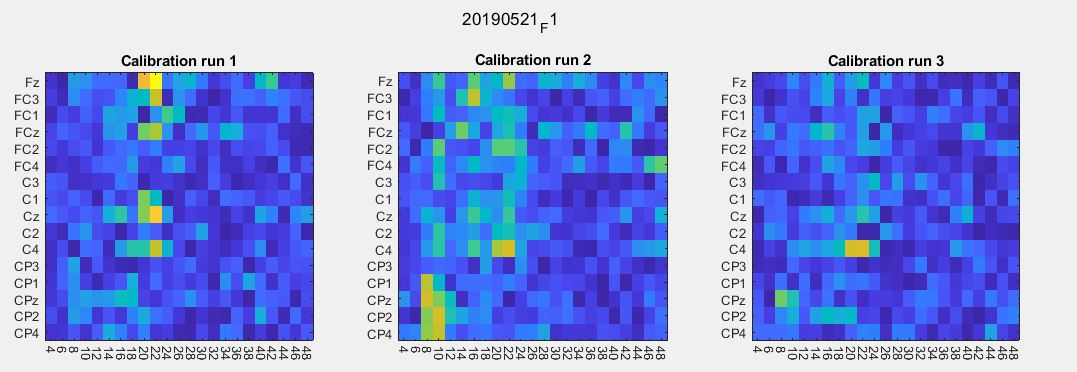
\includegraphics[width=1\textwidth]{Figure/20190521_FS.JPG} }\\
    \multicolumn{2}{c}{(d) 20190521}\\
    \multicolumn{2}{c}{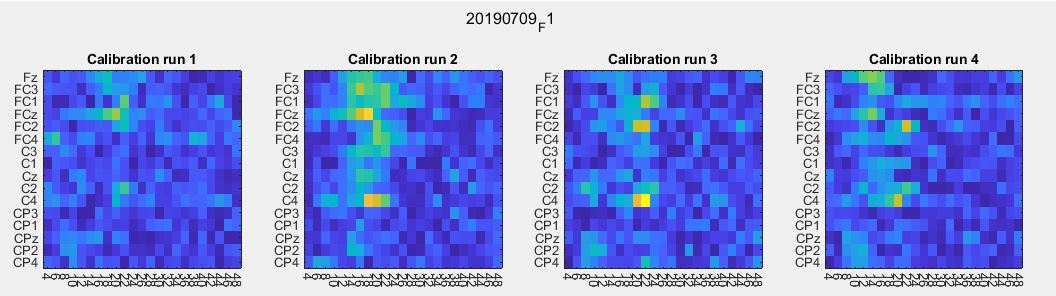
\includegraphics[width=1\textwidth]{Figure/20190709_FS.JPG} }\\
    \multicolumn{2}{c}{(e) 20190709}\\

\end{tabular}
\caption{Fisher score results}
\end{figure}




\begin{figure}
\begin{tabular}{cc}

    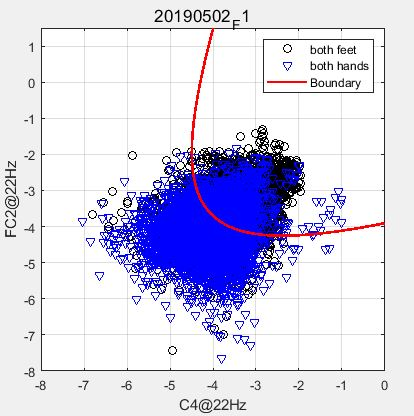
\includegraphics[width=0.5\textwidth]{Figure/20190502_C.JPG} &   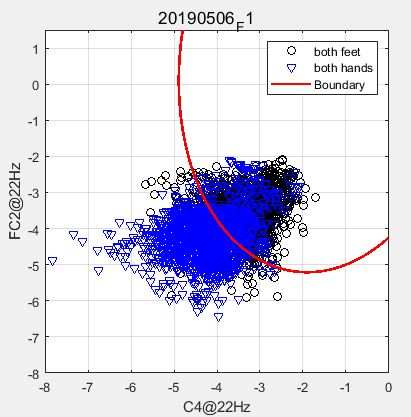
\includegraphics[width=0.5\textwidth]{Figure/20190506_C.JPG} \\
    (a) 20190502 & (b) 20190506 \\
    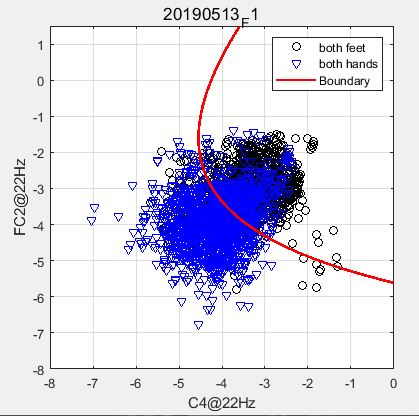
\includegraphics[width=0.5\textwidth]{Figure/20190513_C.JPG} &   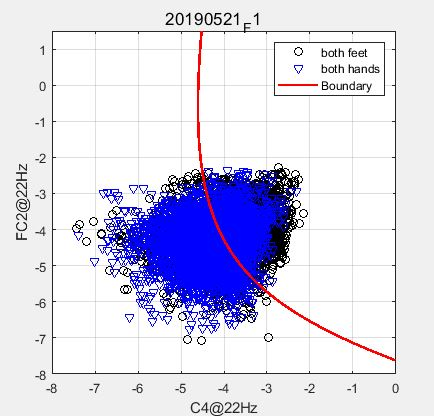
\includegraphics[width=0.5\textwidth]{Figure/20190521_C.JPG} \\
    (c) 20190513 & (d) 20190521 \\
    \multicolumn{2}{c}{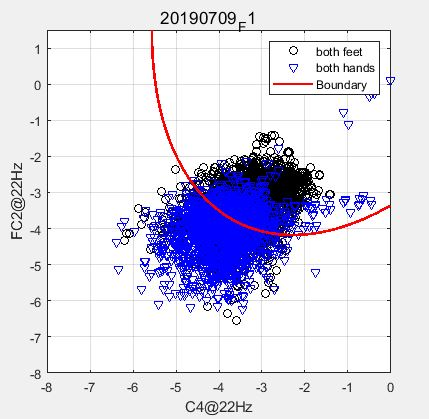
\includegraphics[width=0.5\textwidth]{Figure/20190709_C.JPG} }\\
    \multicolumn{2}{c}{(e) 20190709}\\


\end{tabular}
\caption{Models}
\end{figure}





\begin{figure}
\begin{tabular}{ccc}

    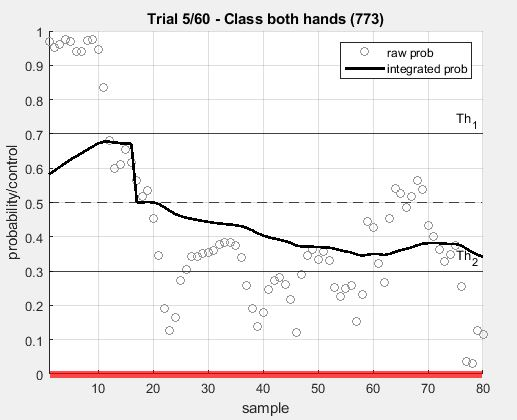
\includegraphics[width=0.3\textwidth]{Figure/20190502_F.JPG} &   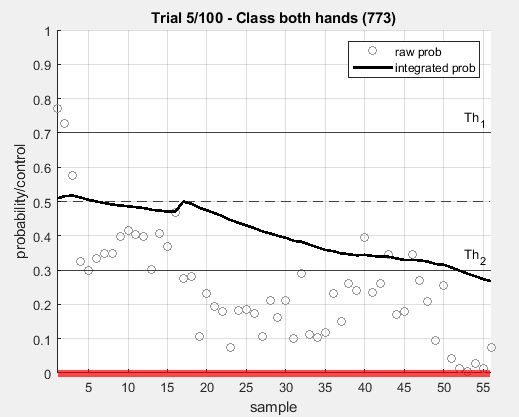
\includegraphics[width=0.3\textwidth]{Figure/20190506_F.JPG}  &   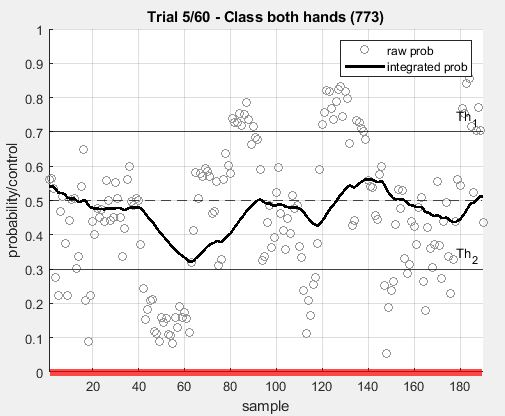
\includegraphics[width=0.3\textwidth]{Figure/20190513_F.JPG} \\
    (a) 20190502 & (b) 20190506 & (c)20190513\\
    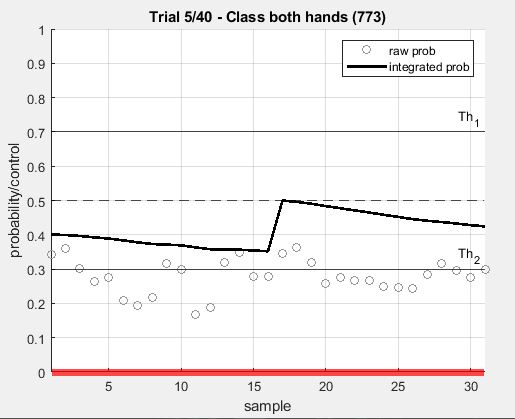
\includegraphics[width=0.3\textwidth]{Figure/20190521_F.JPG} &   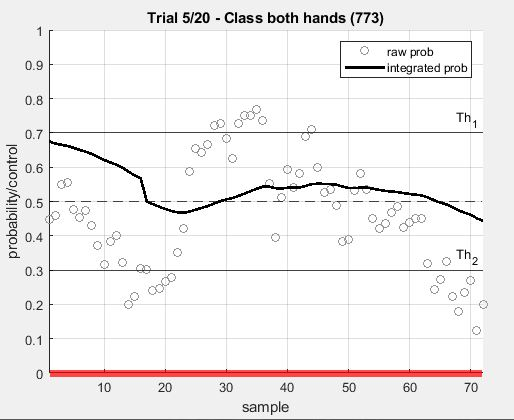
\includegraphics[width=0.3\textwidth]{Figure/20190610_F.JPG}  &   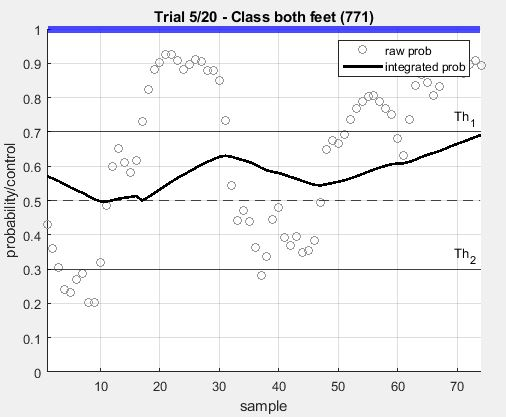
\includegraphics[width=0.3\textwidth]{Figure/20190624_F.JPG} \\
    (d) 20190521 & (e) 20190610 & (f) 20190624 \\
    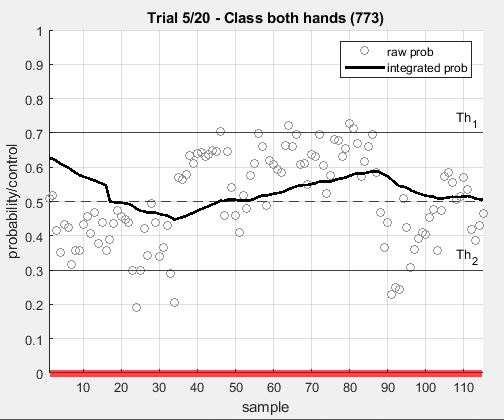
\includegraphics[width=0.3\textwidth]{Figure/20190627_F.JPG} &   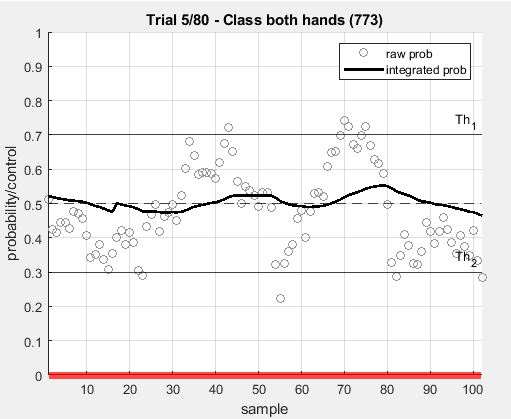
\includegraphics[width=0.3\textwidth]{Figure/20190701_F.JPG}  &   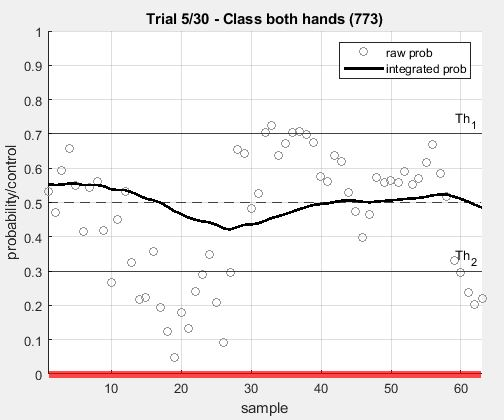
\includegraphics[width=0.3\textwidth]{Figure/20190709_F.JPG} \\
    (g) 20190627 & (h) 20190701 & (i) 20190709 \\
    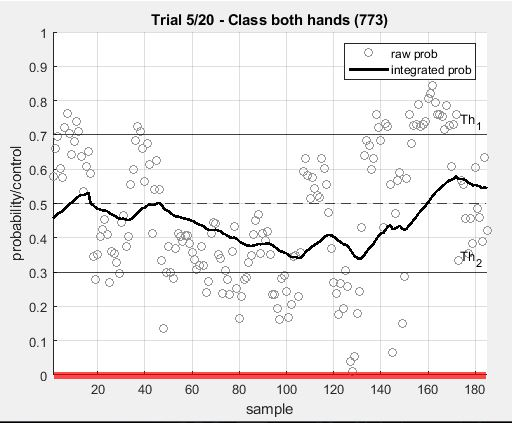
\includegraphics[width=0.3\textwidth]{Figure/20190711_F.JPG} &   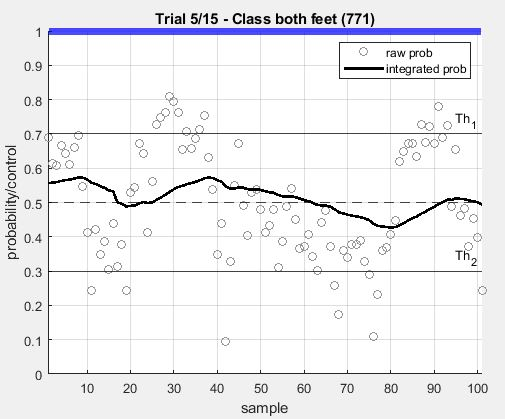
\includegraphics[width=0.3\textwidth]{Figure/20190715_F.JPG}  \\
    (g) 20190711 & (h) 20190715 \\


\end{tabular}
\caption{Models}
\end{figure}






